\begin{subsection}{Events}
% \begin{frame}{Events}
% \begin{itemize}
% 	\item certain conditions trigger instantaneous changes in state variables
%     \item example: bouncing ball
% \end{itemize}
%   \begin{figure}
%   	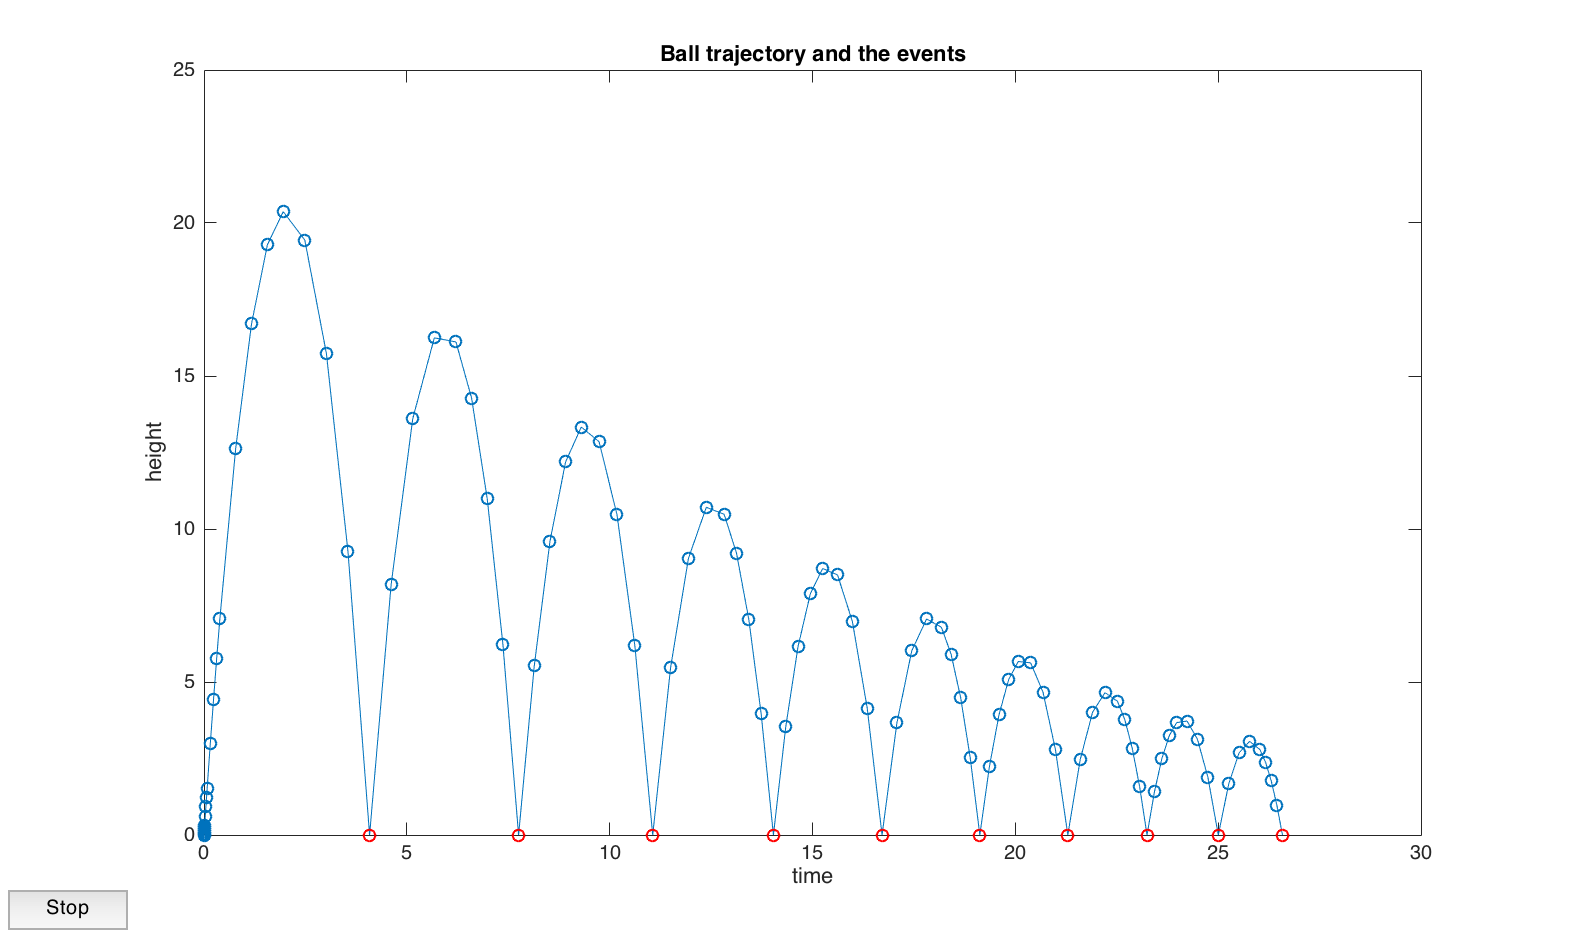
\includegraphics[height=5cm]{images/bouncing-ball}
%     \caption{Matlab ballode example}
%   \end{figure}
% \end{frame}

% \begin{frame}{Events}
% uses:
% \begin{itemize}
% 	\item ``bouncing'' ants off the arena walls
% 	\item switching between forager and returner roles
%   \item random reorientation events

% \end{itemize}
% \end{frame}

\begin{frame}{Random Reorientation Events \scriptsize{\cite{khuong_how_2013}}}
\begin{columns}[T,onlytextwidth]
\column{0.45\textwidth}
\begin{align*}
\frac{d}{dt} \begin{pmatrix}\vec{x}\\\vec{v}\\s\end{pmatrix} = \begin{pmatrix}\ldots \\ \ldots\\ \norm{v}\end{pmatrix}
\end{align*}
\column{0.1\textwidth}
\column{0.45\textwidth}
\begin{align*}
\theta_{\operatorname{new}} = \theta_{\operatorname{old}} + \bm{T} \\
s = 0 \\
s_{\operatorname{thresh}} = \bm{X}
\end{align*}
\end{columns}
\vspace{-2ex}
\begin{figure}
	\begin{columns}[T, onlytextwidth]
		\column{0.1\textwidth}
		\column{0.4\textwidth}
		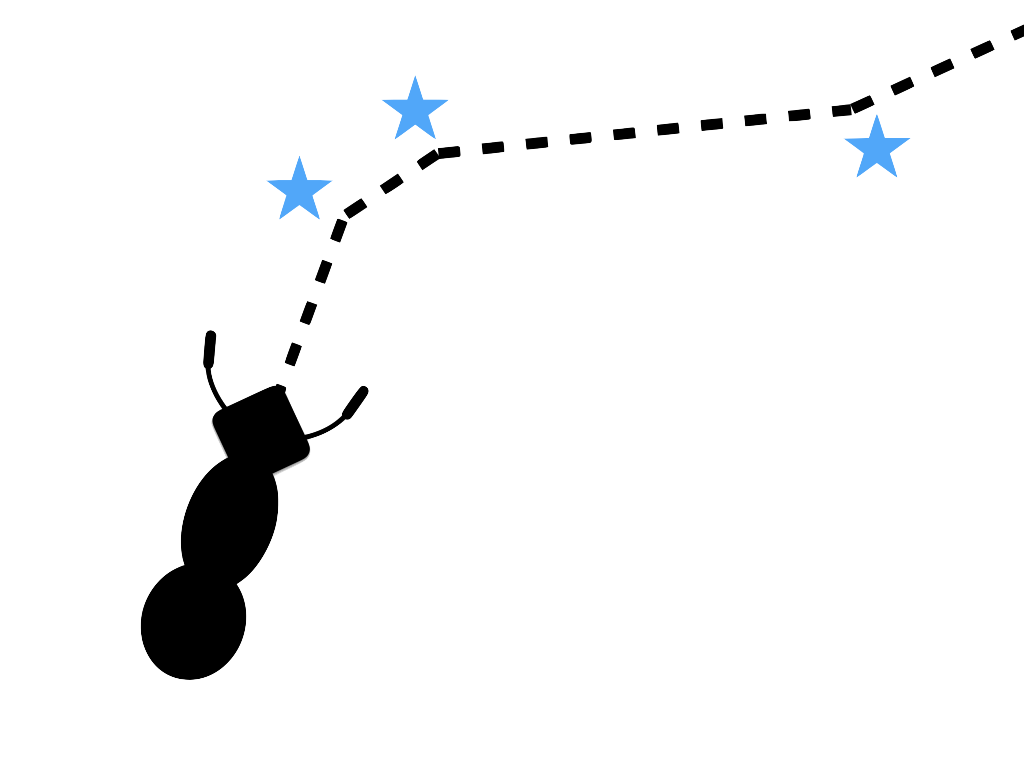
\includegraphics[width=\textwidth]{images/model_components_cartoons_009}
		\column{0.4\textwidth}
		\caption{\footnotesize{``Boltzmann walker'' cartoon; blue stars denote random reorientation events}}
		\column{0.1\textwidth}
	\end{columns}
\end{figure}
\vspace{-6ex}
\begin{itemize}
		%\item ant ``keeps track'' of how far it has traveled, $s$
    \item upon reaching a threshold distance ($s > s_{\operatorname{thresh}}$), the ant experiences a ``reorientation event''
    \item the threshold distance is generated from an exponential distribution %($\bm{X} \sim \mathit{exp}(\omega)$)
    %\item ``memoryless property'' (probability of reorientation is uniform over every unit of distance the ant traverses)
    \item the angle the ant turns through is normally distributed % ($\Delta \theta = \bm{T} \sim \mathcal{N}(0,\sigma^2)$)
\end{itemize}
\end{frame}

\begin{frame}{Random Reorientation Events: Adjustments}
\begin{columns}[T,onlytextwidth]

\column{0.6\textwidth}
\begin{figure}
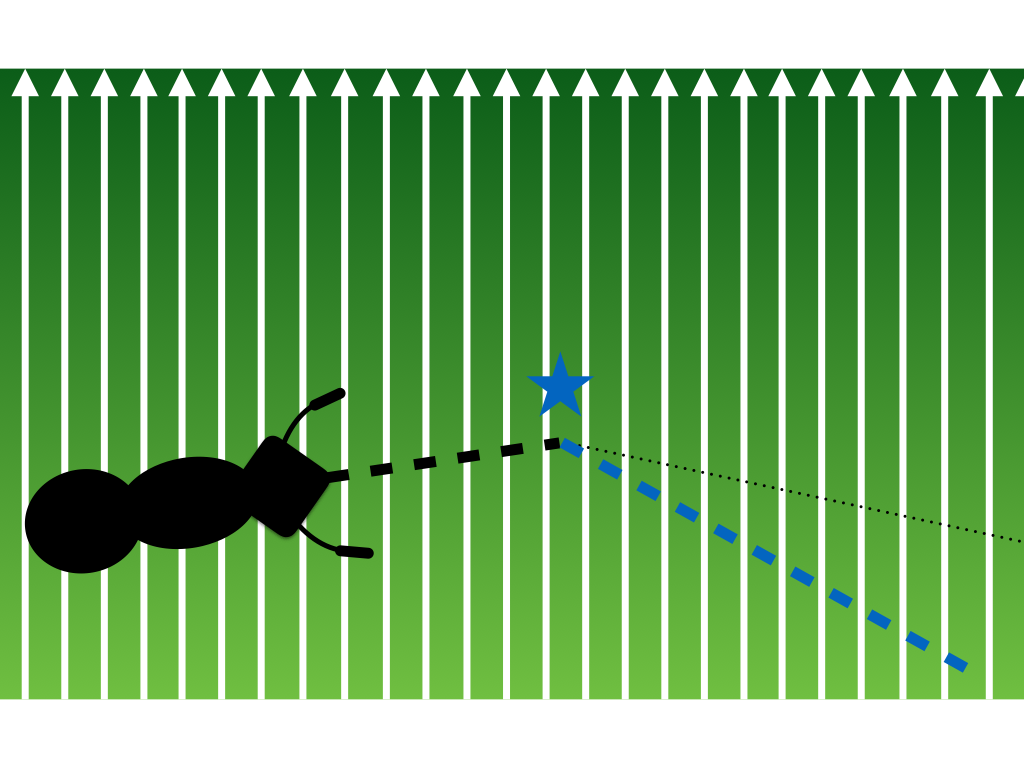
\includegraphics[width=0.6\textwidth]{images/model_components_cartoons_012}
\vspace{-2ex}
\caption{
\footnotesize{Illustration of adjustment accounting for ant behavior on uneven terrain}}
\end{figure}
\column{0.4\textwidth}
\begin{align*}
\bm{T}_{\operatorname{effective}} = \bm{T} / \beta \\
\beta =
\begin{cases}
      \text{forager role} & e^{c_1p} \\
      \text{returner role} & c_2
\end{cases} \\
s_{\operatorname{thresh}} = \bm{X} + c_3 \frac{|\vec{s} \cdot \vec{v}|}{\norm{\vec{v}}}
\end{align*}

\end{columns}
\begin{itemize}
  \item free path of ant ($s_{\operatorname{thresh}}$) increases if ant oriented with or against the gradient {\scriptsize\cite{khuong_how_2013}}
  \item ants preferentially re-orient themselves to align with or against a surface's topographical gradient {\scriptsize\cite{khuong_how_2013}}
	\item severity of random reorientation decreased when following pheromone trail and returning to nest
\end{itemize}
\end{frame}

% \begin{frame}{Events}
% \alert{behavioral effect of incline:}
% \begin{itemize}
% \end{itemize}
% \begin{columns}[T,onlytextwidth]
% \column{\textwidth}

% \begin{figure}
% \begin{minipage}[]{0.3\textwidth}
%     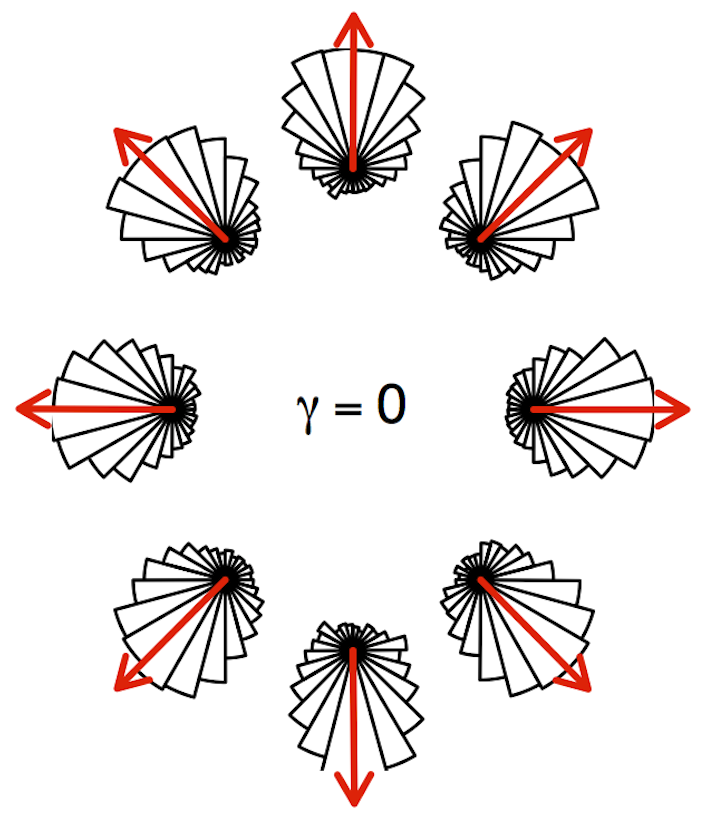
\includegraphics[width=\textwidth]{images/khuong_0}
% \end{minipage}%
% \begin{minipage}[]{0.05\textwidth}
% ~
% \end{minipage}%
% \begin{minipage}[]{0.3\textwidth}
%     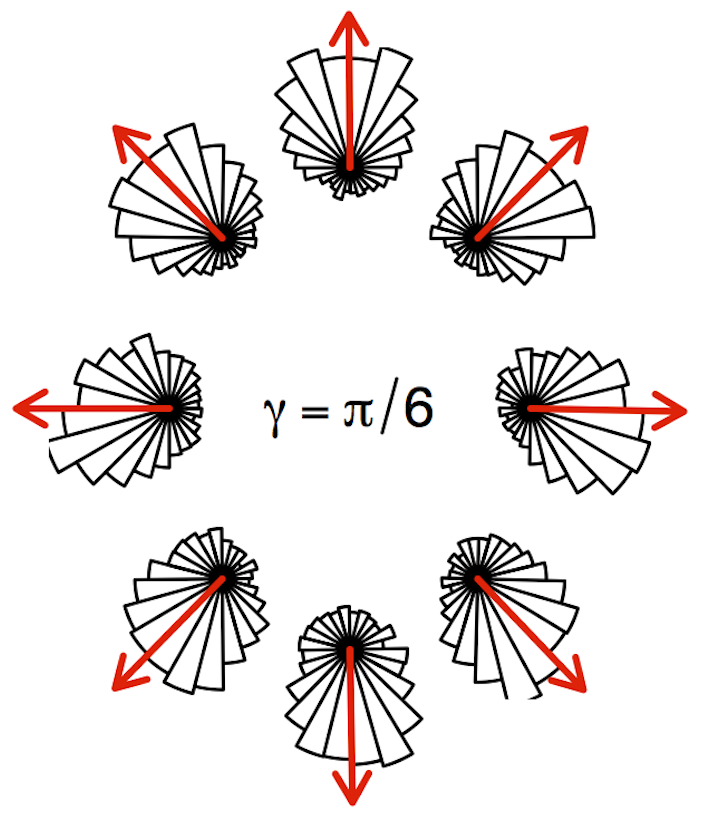
\includegraphics[width=\textwidth]{images/khuong_pi_div_6}
% \end{minipage}%
% \begin{minipage}[]{0.05\textwidth}
% ~
% \end{minipage}%
% \begin{minipage}[]{0.3\textwidth}
%     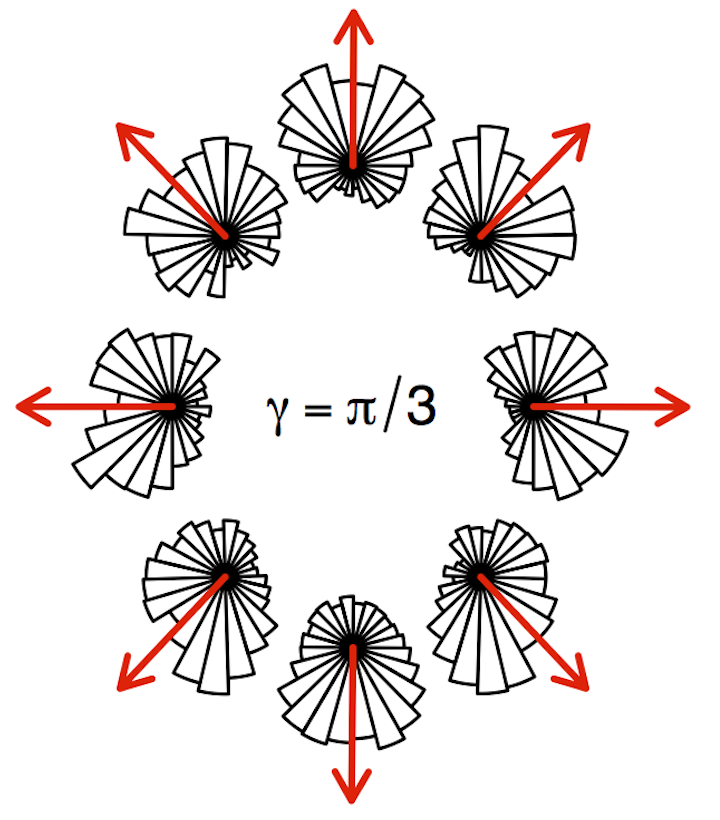
\includegraphics[width=\textwidth]{images/khuong_pi_div_3}
% \end{minipage}%
% \caption{Ant Reorientation on Inclined Surfaces \scriptsize{\cite{khuong_how_2013}}}
% \end{figure}
% \end{columns}

% \end{frame}

\end{subsection}
